\section{Mean SIC with different indicies}
\begin{table}[H]
\begin{tabular}{@{}rllll@{}}
\toprule
                                      & \textbf{SAM} & \textbf{IPO} & \textbf{DMI} & \textbf{ENSO} \\ \midrule
\textbf{raw monthly}                  & -0.0286      & -0.02356     & 0.149673     & -0.02178      \\
\textbf{raw monthly detrended}        & -0.03614     & -0.01259     & 0.14486      & -0.02917      \\
\textbf{anomalous monthly}            & \textbf{0.153142}     & \textbf{-0.12784}     & 0.112879     & 0.067515      \\
\textbf{anomalous monthly detrended}  & \textbf{0.117848}     & -0.06747     & 0.113995     & 0.02886       \\
\textbf{raw seasonal}                 & -0.04518     & -0.0298      & 0.05791      & -0.01521      \\
\textbf{raw seasonal detrended}       & -0.06096     & -0.0148      & 0.055534     & -0.02615      \\
\textbf{anomalous seasonal}           & \textbf{0.191653}     & -0.14036     & 0.026778     & 0.092851      \\
\textbf{anomalous seasonal detrended} & 0.131356     & -0.06952     & 0.006859     & 0.043756      \\
\textbf{raw annual}                   & 0.270046     & -0.13599     & 0.014287     & 0.115359      \\
\textbf{raw annual detrended}         & 0.13903      & -0.02698     & -0.02919     & 0.028031      \\
\textbf{anomalous annual}             & 0.278939     & -0.16029     & 0.014941     & 0.135027      \\
\textbf{anomalous annual detrended}   & 0.144474     & -0.05059     & -0.03012     & 0.046729      \\ \bottomrule
\end{tabular}
\caption{Correlations between different indices and SIC in Antarctica. Bold values indicate statistical significance i.e. a p-value lower than 0.05.}
\end{table}

% Please add the following required packages to your document preamble:
% \usepackage{booktabs}
\begin{table}[H]
\begin{tabular}{@{}rllll@{}}
\toprule
                                      & \textbf{SAM} & \textbf{IPO} & \textbf{DMI} & \textbf{ENSO} \\ \midrule
\textbf{raw monthly}                  & 0.53     & 0.60     & 0.24     & 0.63      \\
\textbf{raw monthly detrended}        & 0.43     & 0.78     & 0.25     & 0.52      \\
\textbf{anomalous monthly}            & 0.00     & 0.00     & 0.37     & 0.14      \\
\textbf{anomalous monthly detrended}  & 0.00     & 0.14     & 0.37     & 0.52      \\
\textbf{raw seasonal}                 & 0.57     & 0.70     & 0.48     & 0.84      \\
\textbf{raw seasonal detrended}       & 0.44     & 0.85     & 0.50     & 0.74      \\
\textbf{anomalous seasonal}           & 0.01     & 0.07     & 0.74     & 0.24      \\
\textbf{anomalous seasonal detrended} & 0.09     & 0.38     & 0.93     & 0.58      \\
\textbf{raw annual}                   & 0.09     & 0.40     & 0.93     & 0.47      \\
\textbf{raw annual detrended}         & 0.39     & 0.86     & 0.86     & 0.86      \\
\textbf{anomalous annual}             & 0.08     & 0.32     & 0.92     & 0.40      \\
\textbf{anomalous annual detrended}   & 0.37     & 0.75     & 0.85     & 0.77      \\ \bottomrule
\end{tabular}
\caption{p-values for the above correlations.}
\end{table}

\section{Annually averaged results}
For the annually averaged time series, no time-shift was included and there is no difference between the raw and anomalous datasets so we only have two plots, one with the trend and one without.
\begin{figure}[H]
    \centering
    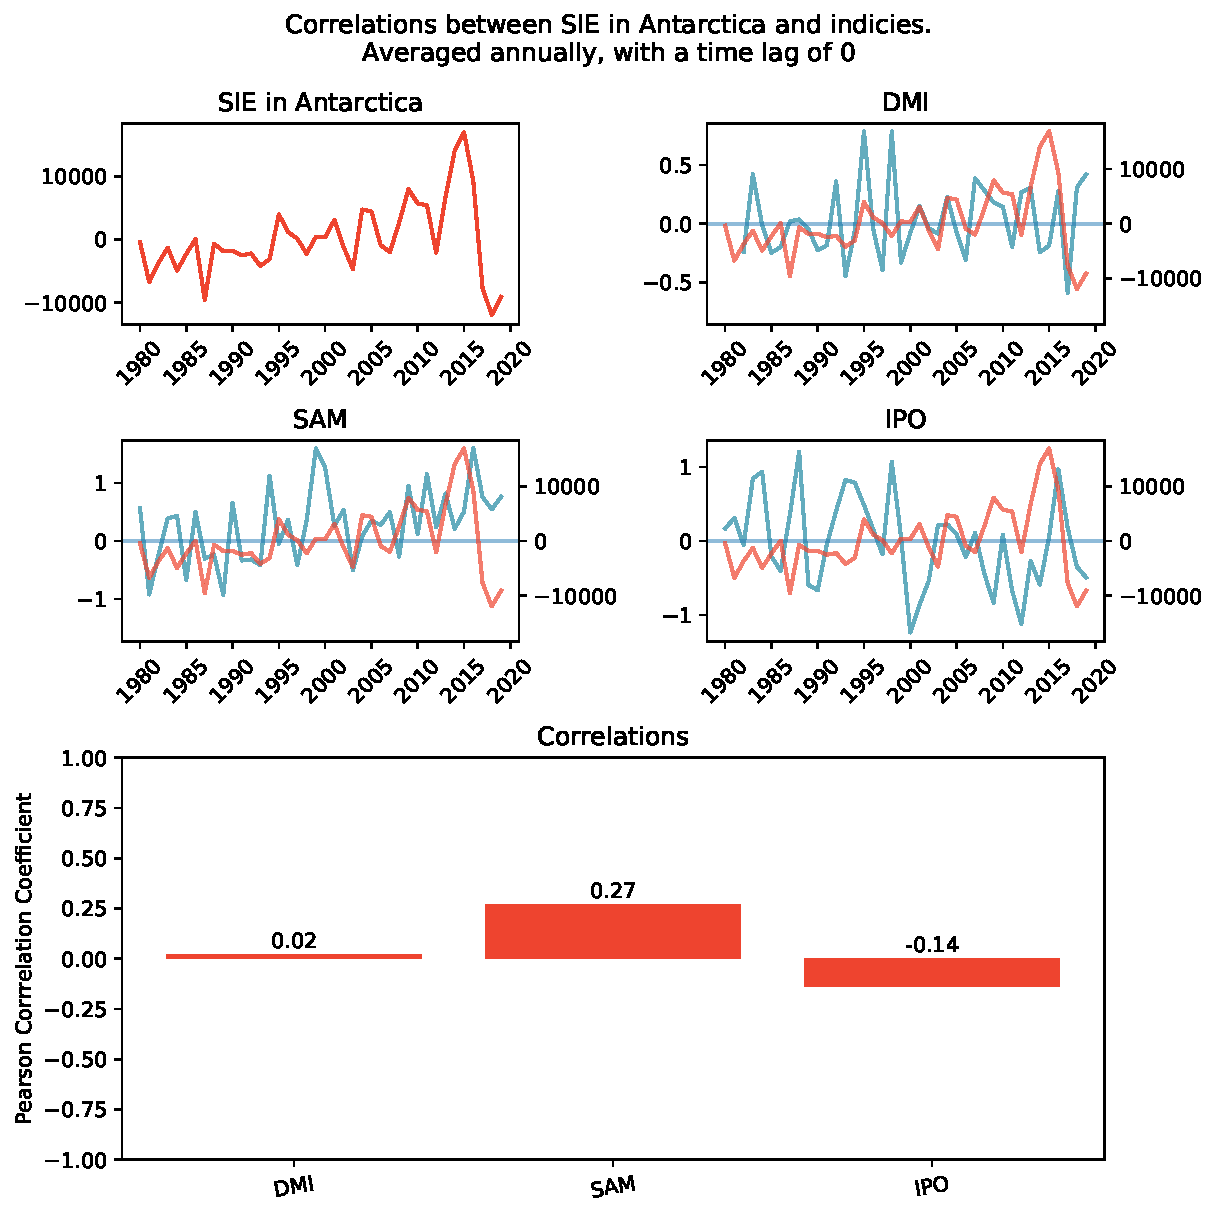
\includegraphics[width=\linewidth]{Images_3.0/correlations/subplots_indicies_annually_0_anomalous.pdf}
    \caption[Correlations between SIE in Antarctica and indices, averaged annually with no time lag.]{Correlations between SIE in Antarctica and indices, averaged annually with no time lag. The first 4 plots are time series of total SIE and the different indices so we can visually gain an understanding regarding the correlations. The bottom plot is a bar plot showing the correlations between SIE and the different indices. Blue bars have a p-value less than 0.05 and are considered statistically significant. Red bars have a p-value larger than 0.05 and are considered statistically insignificant.}
    \label{fig:anual_with_trend}
\end{figure}

\begin{figure}[H]
    \centering
    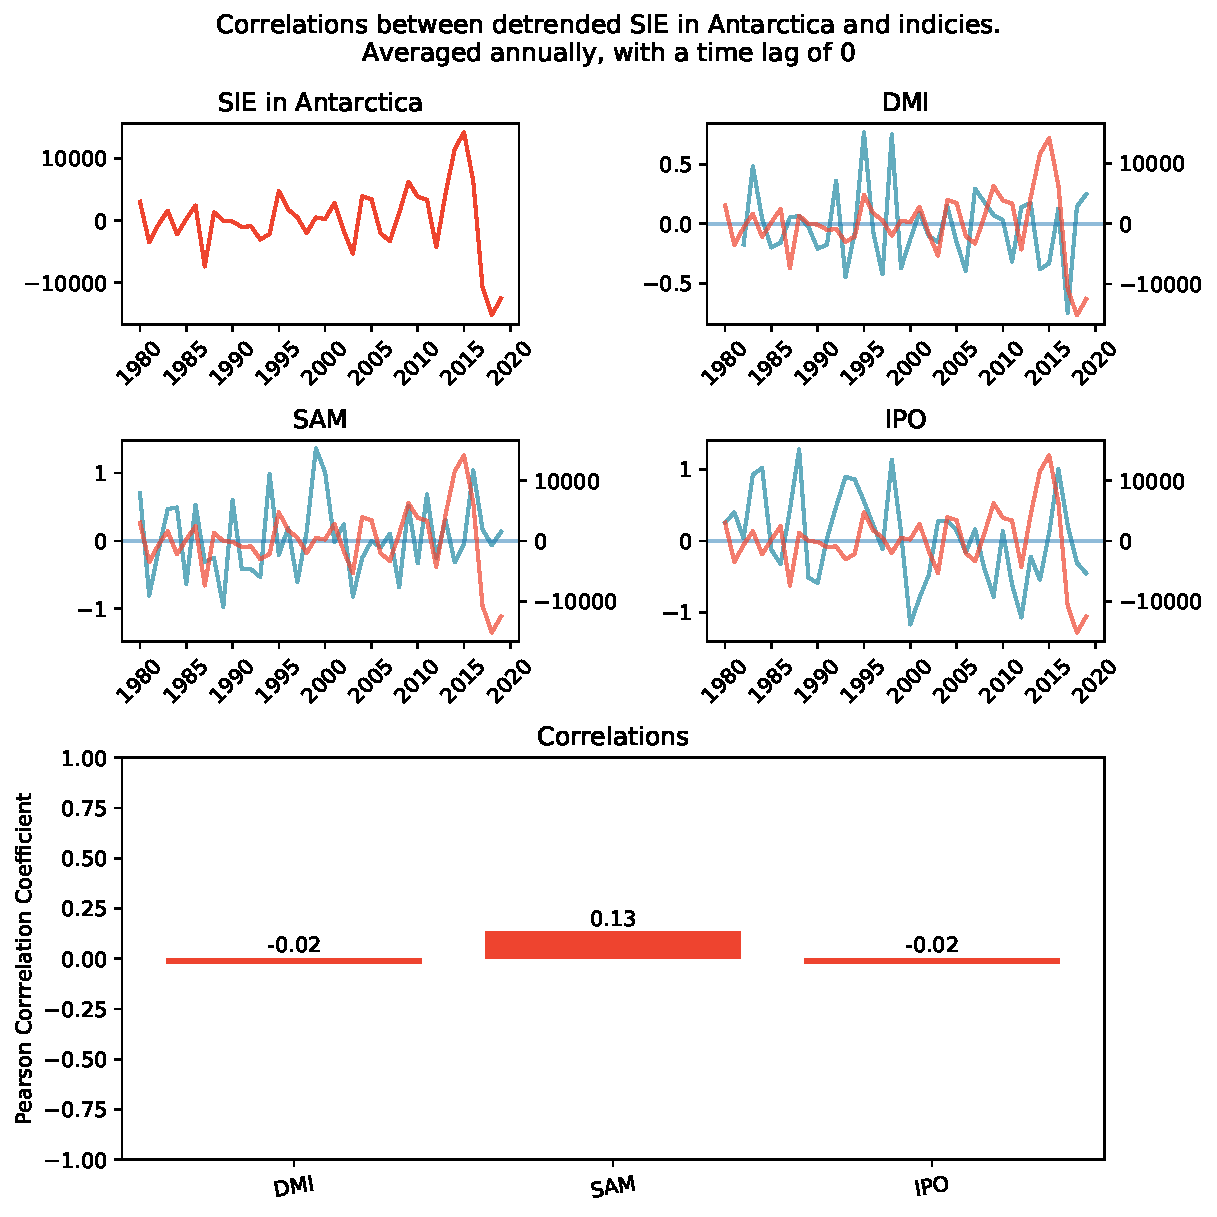
\includegraphics[width=\linewidth]{Images_3.0/correlations/subplots_indicies_annually_0_anomalous_detrended.pdf}
    \caption[Correlations between SIE in Antarctica and indices, averaged annually and detrended with no time lag.]{Correlations between SIE in Antarctica and indices, averaged annually and detrended with no time lag. The first 4 plots are time series of total SIE and the different indices so we can visually gain an understanding regarding the correlations. The bottom plot is a bar plot showing the correlations between SIE and the different indices. Blue bars have a p-value less than 0.05 and are considered statistically significant. Red bars have a p-value larger than 0.05 and are considered statistically insignificant.}
    \label{fig:annual_without_trend}
\end{figure}
Not much can be said from the above figures as all the correlations are insignificant. This could be for a number of reasons, not least because we are only looking at 40 data-points for each time series or that we are considering the behaviour of ice over a large spatial area. Though still statistically insignificant, the correlations are larger for the case where the trend is included.


\section{Monthly averages}

In order to hopefully gain better results, we looked at this with a higher temporal resolution (monthly rather than annually averaged). This has the advantage of picking up higher frequency behaviours, but also is more noisy as a result. Additionally with the higher resolution it makes sense to explore lead-lag relationships between the different variables, this is something we do later in this thesis.


\begin{figure}[H]
    \centering
    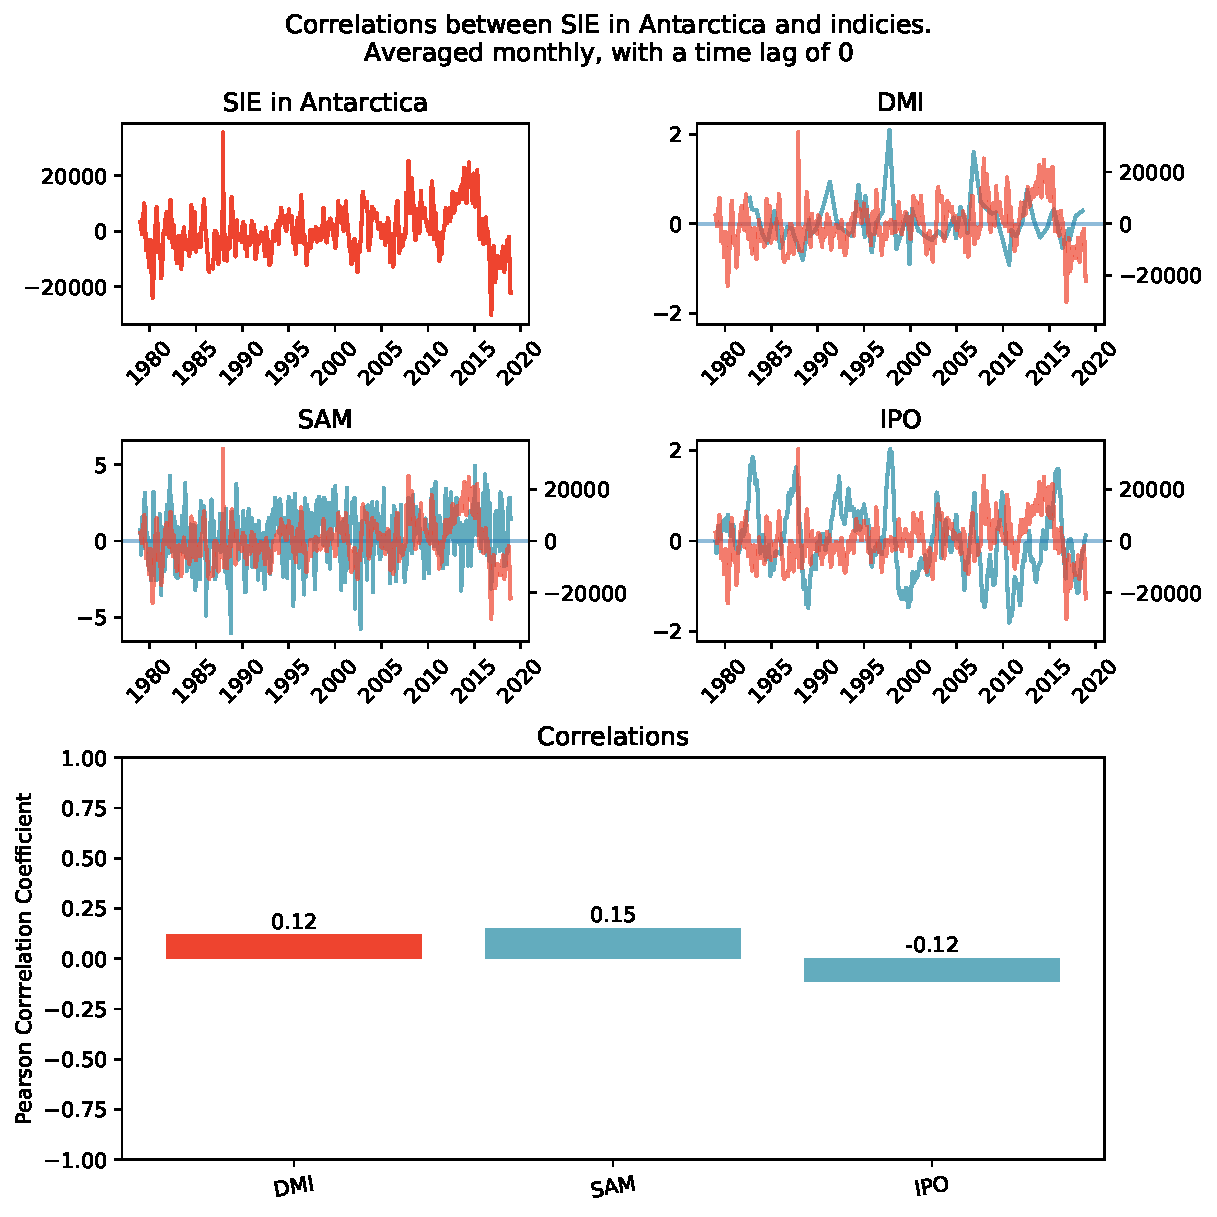
\includegraphics[width = \linewidth]{Images_3.0/correlations/subplots_indicies_monthly_0_anomalous.pdf}
    \caption[Correlations between SIE in Antarctica and indices, averaged monthly with no time lag.]{Correlations between SIE in Antarctica and indices, averaged monthly with no time lag. The first 4 plots are time series of total SIE and the different indices so we can visually gain an understanding regarding the correlations. The bottom plot is a bar plot showing the correlations between SIE and the different indices. Blue bars have a p-value less than 0.05 and are considered statistically significant. Red bars have a p-value larger than 0.05 and are considered statistically insignificant.}
    \label{fig:seasonal_with_trend}
\end{figure}
Immediately, this figure tells us that SAM and IPO both have significant correlations with SIE in Antarctica on a monthly basis. For SAM this is unsurprising as the pattern is defined as changes in wind speeds and pressures at the high southern latitudes close to Antarctica \textcolor{red}{(get proper definition and cite}. For IPO this is also makes some sense as it is a major climate signal over the Pacific. \textcolor{red}{Do other people get the same result?} To help build our understanding of these relationships, let's look at what happens when we detrend the time series.

\begin{figure}[H]
    \centering
    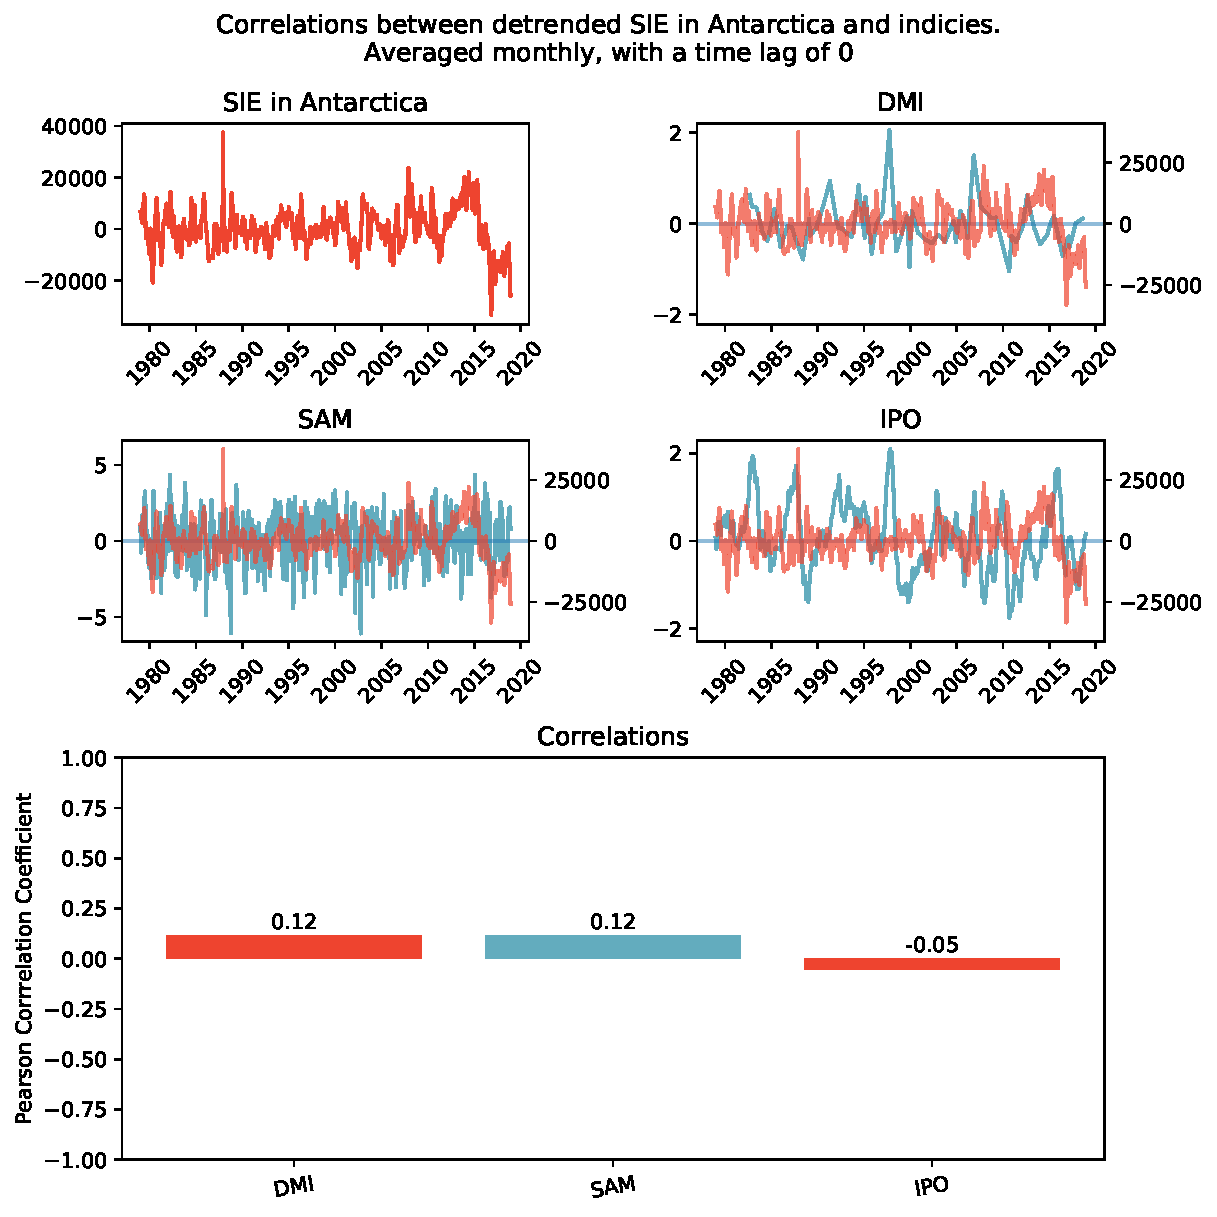
\includegraphics[width = \linewidth]{Images_3.0/correlations/subplots_indicies_monthly_0_anomalous_detrended.pdf}
    \caption[Correlations between SIE in Antarctica and indices, averaged monthly, detrended with no time lag.]{Correlations between SIE in Antarctica and indices, averaged monthly, detrended with no time lag. The first 4 plots are time series of total SIE and the different indices so we can visually gain an understanding regarding the correlations. The bottom plot is a bar plot showing the correlations between SIE and the different indices. Blue bars have a p-value less than 0.05 and are considered statistically significant. Red bars have a p-value larger than 0.05 and are considered statistically insignificant.}
    \label{fig:seasonal_without_trend}
\end{figure}

When we remove the trend the magnitude of the correlations decrease for SAM and IPO, whereas DMI has no change in the magnitude of correlation. The correlation between SAM and SIE in Antarctica remains statistically significant whereas the IPO is no longer significant. 


\section{Lead lag analysis for monthly data}

We can perform some lead-lag analysis on the correlations between the different indices and SIE in Antarctica, to gain some understanding on if there are any delayed signals of significance we need to consider. Because the indices are initially anomalous signals, we only did this for the anomalous sea ice data. In the following plots, a negative time-lag indicates that we are comparing the time-series for sea ice with patterns in each index before that point. A positive time-lag indicates that we are comparing the time-series for sea ice with patterns in each index after that point. The size of the time-lag indicates the length to which the sea ice time series was shifted.
\begin{figure}[H]
    \centering
    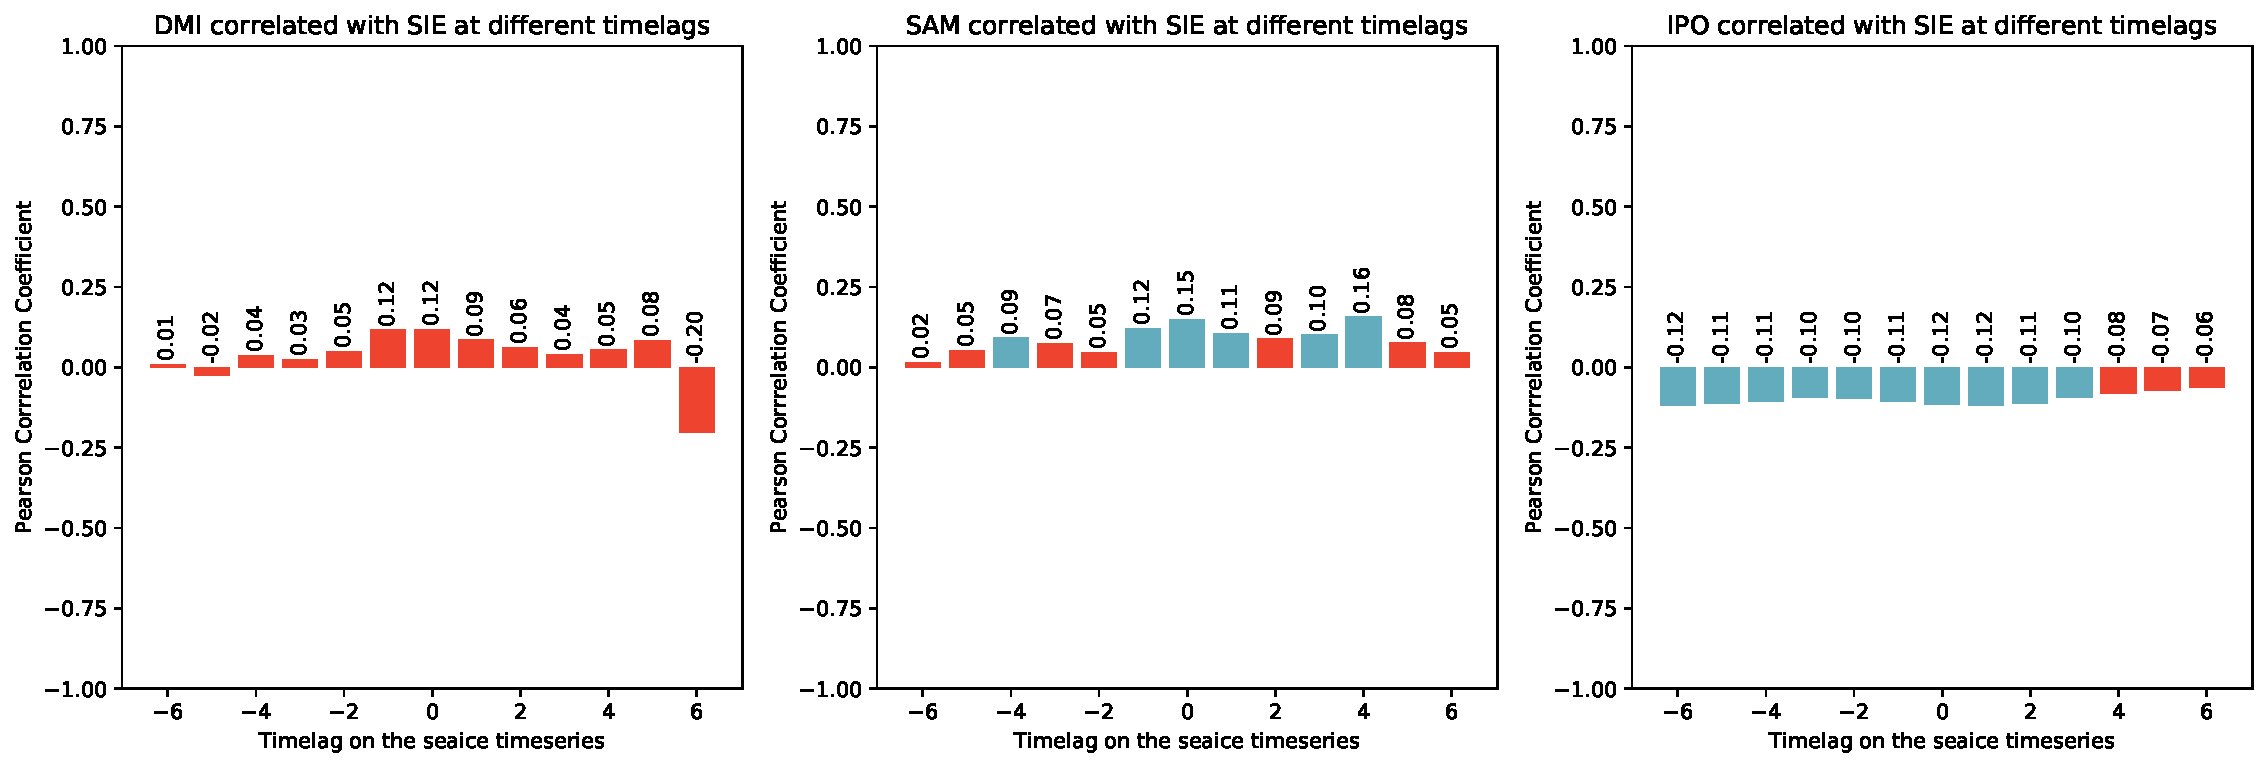
\includegraphics[width = \linewidth]{Images_3.0/correlations/indicies_monthly_anomalous.pdf}
    \caption[Histograms of correlations with different indices at different time-lags with anomalous Antarctic SIE.]{Histograms of correlations with different indices at different time-lags with anomalous Antarctic SIE. A blue bar indicates a statistically significant p-value of less than 0.05. A red bar indicates a statistically insignificant value.}
    \label{fig:leadlag_anomalous}
\end{figure}

DMI has no significant correlation with Antarctic SIE regardless of time-lag. SAM has a significant correlation for time-lags of -1, 0, 1, 3, 4, and 5 months. IPO has significant correlations for any time-lag less than 3 months (including negative time-lags). It's possible that the trend is confusing the signals here so let's see what happens when we remove it.

\begin{figure}[H]
    \centering
    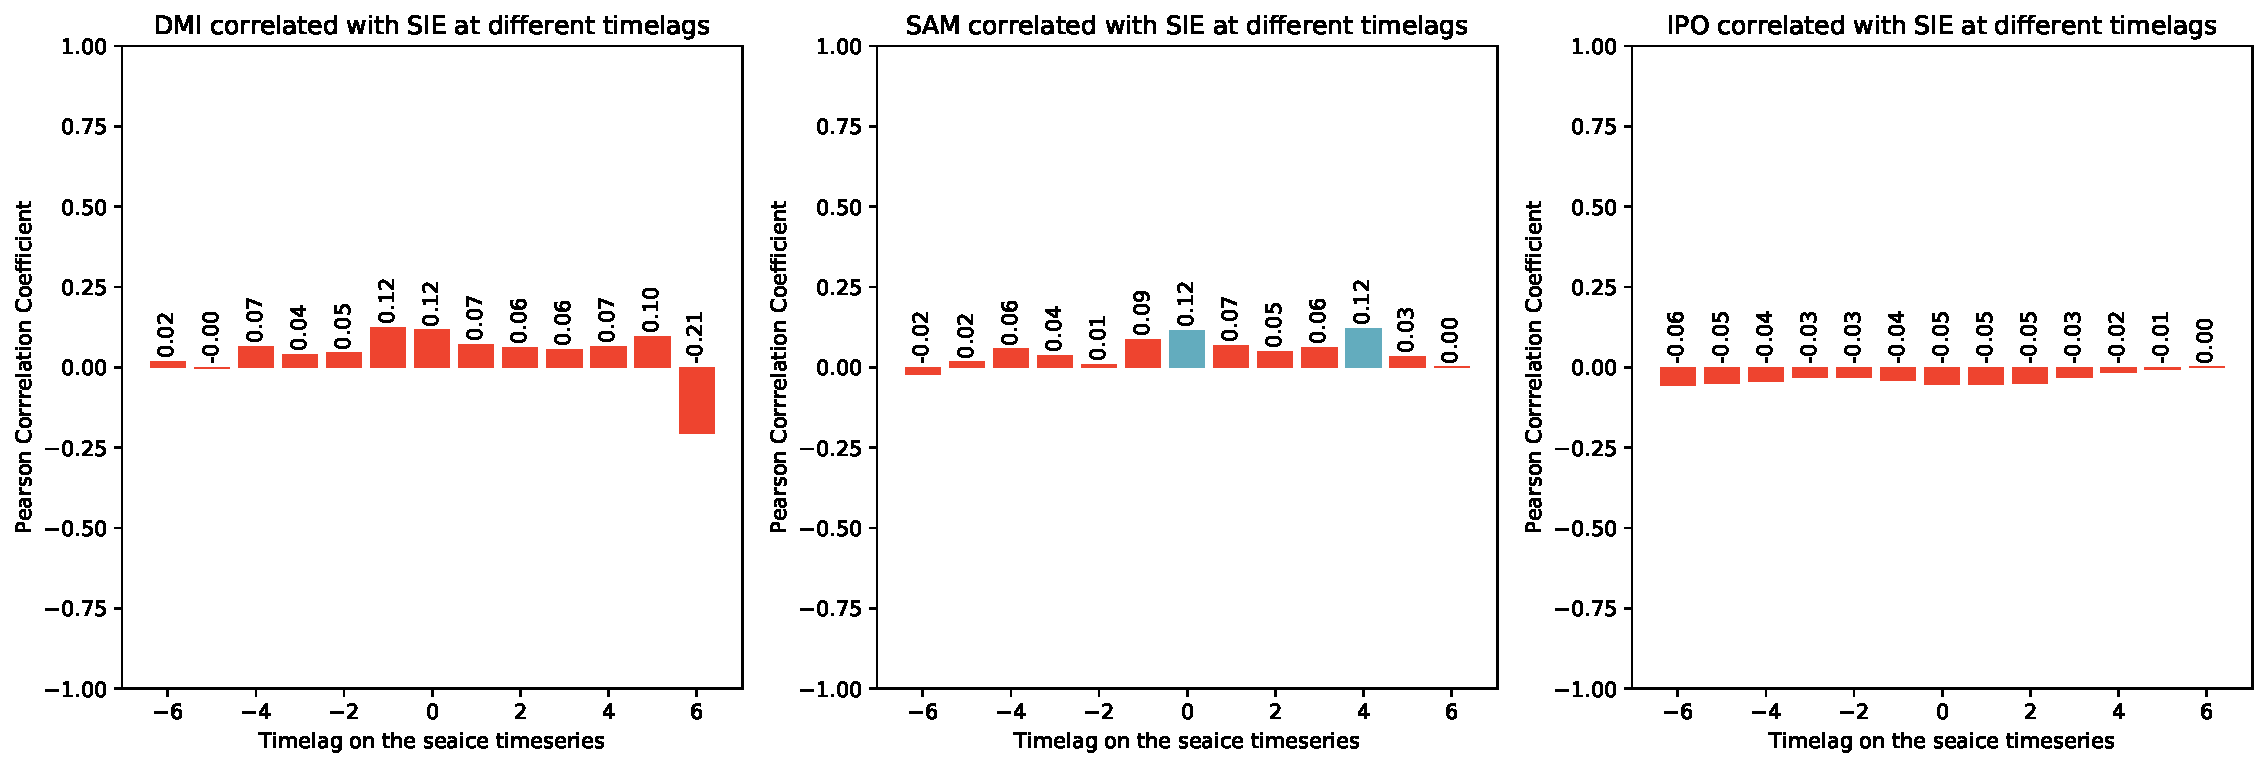
\includegraphics[width = \linewidth]{Images_3.0/correlations/indicies_monthly_anomalous_detrended.pdf}
    \caption[Histograms of correlations with different indices at different time-lags with anomalous and detrended Antarctic SIE.]{Histograms of correlations with different indices at different time-lags with anomalous and detrended Antarctic SIE. A blue bar indicates a statistically significant p-value of less than 0.05. A red bar indicates a statistically insignificant value.}
    \label{fig:leadlag_anomalous_detrended}
\end{figure}

The only significant correlations we observe at this point are the correlations between SAM and Antarctic SIE for time-lags of 0 and 4 months. This indicates that when an event occurs for Antarctic SIE, it is likely that we would observe a related event in the SAM index at the same time and also 4 months later. \textcolor{red}{not sure if I worded this right so let's go with it for now.}\medskip

One problem we have here is that we are not totally able to use the information for the correlations which we have above to inform us regarding how events for the different indexed circulations could potentially impact the behaviour of sea ice we see in Antarctica. For that we want to look at the first time derivative of Antarctic SIE to see if it has behaviours related to these indices.